\structure{ХОД РАБОТЫ}

В проекте был написан класс для решения позиционных игр методом обратной индукции. Также
был реализован алгоритм построения деревьев с большой глубиной при помощи языка для
отрисовки графов Dot.

Пример запуска программы:

\begin{codelisting}[language=Bash]
    go run cmd/lw4/main.go
\end{codelisting}

Решим позционную игру методом обратной индукции.


\section{Метод обратной индукции}

В динамических играх с полной и совершенной информацией удобно решать игру методом
обратной индукции. В методе обратной индукции рассматриваются все последние вершины игры,
в которых один из игроков делает выбор, исходя из его рациональности. Далее процесс
повторяется для всех предшествующих вершин, пока не дойдет до начальной вершины.

Для решения сгенерируем дерево, согласно таблице~\ref{tab:tab01}. Так как дерево слишком
большое, далее будут представлены его части, в которых берутся выигрышные стратегии от
листовых узлов до корня.

\begin{figure}
  \centering
  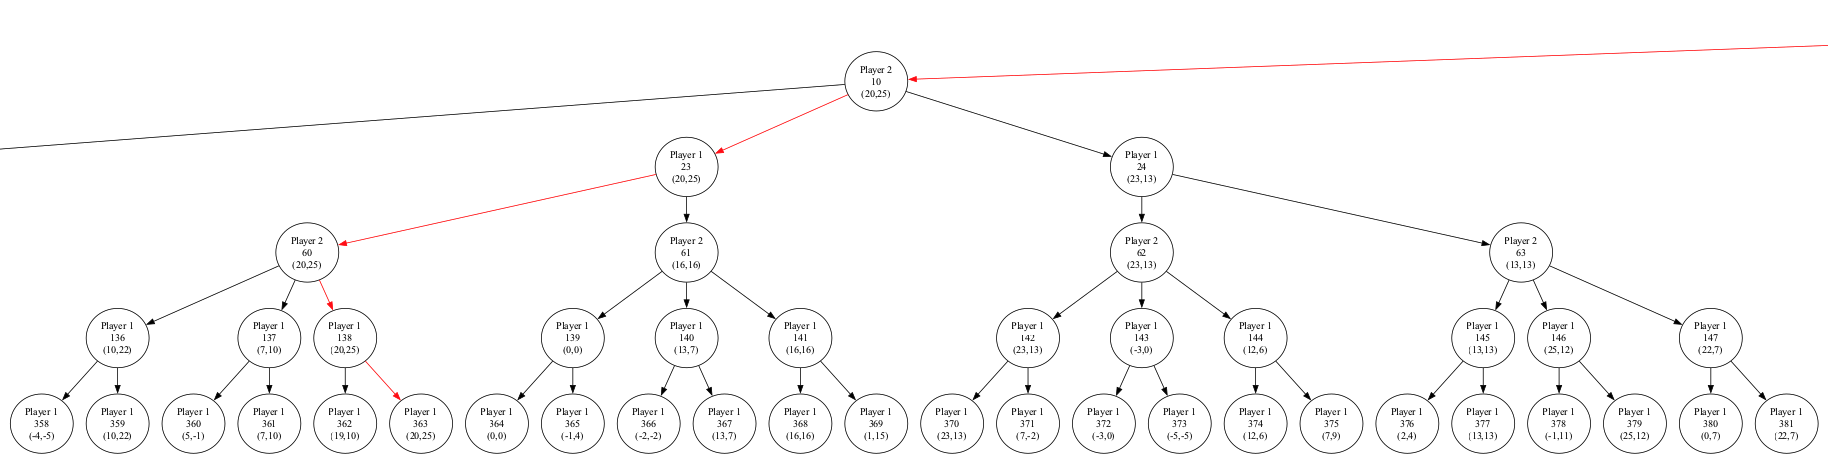
\includegraphics[scale=0.3]{../../artifacts/lw4/1.png}
  \caption{Нижний уровень дерева}
  \label{fig:fig01}
\end{figure}

На рисунке~\ref{fig:fig01} покрашены красным цветом ребра графа, по которому идет
выигрышная стратегия. Например, между 362 и 363 узлом выбирается 363, так как при ходе
первого игрока кортеж (20, 25) больше (19, 10).

\begin{figure}
  \centering
  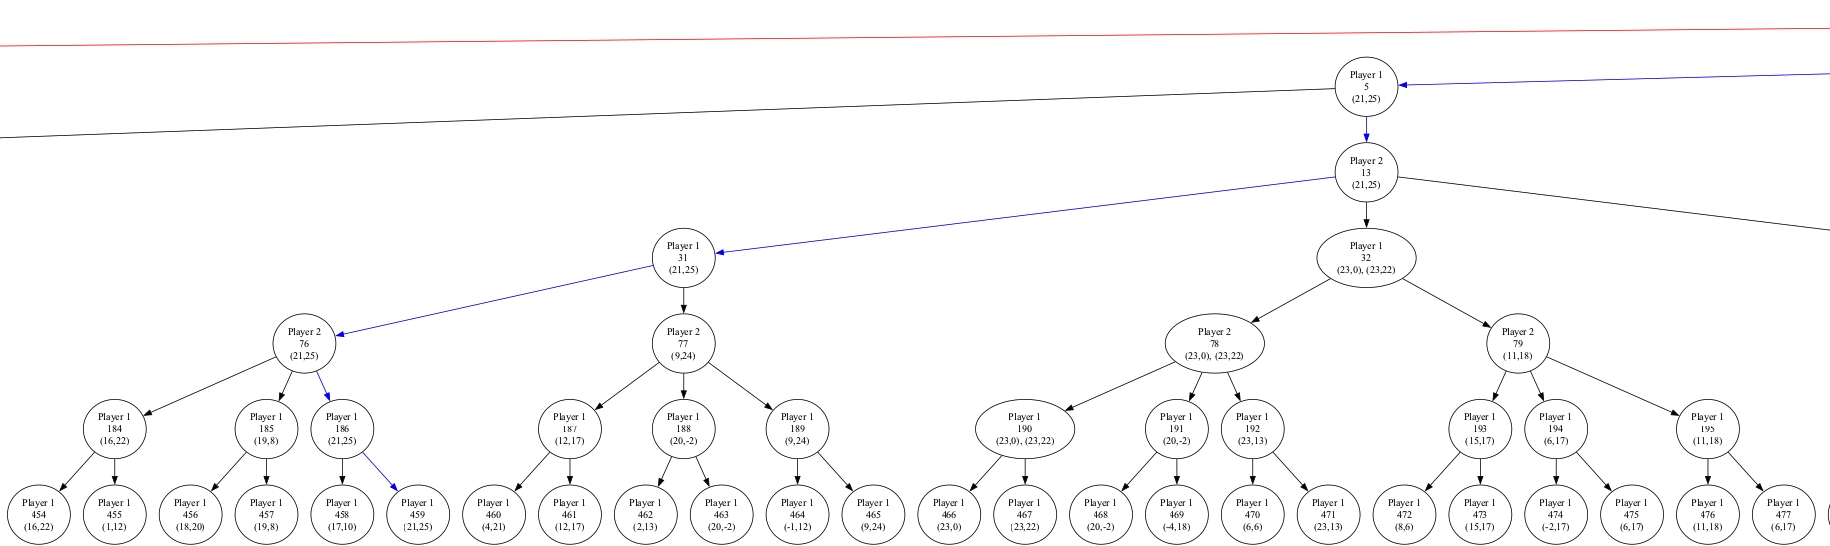
\includegraphics[scale=0.3]{../../artifacts/lw4/2.png}
  \caption{Промежуточная индукция}
  \label{fig:fig02}
\end{figure}

На рисунке~\ref{fig:fig02} покрашены синим цветом ребра гарафа другой равновероятной
стратегии. Проталкивание кортежа вверх производится аналогичным образом.

\begin{figure}
  \centering
  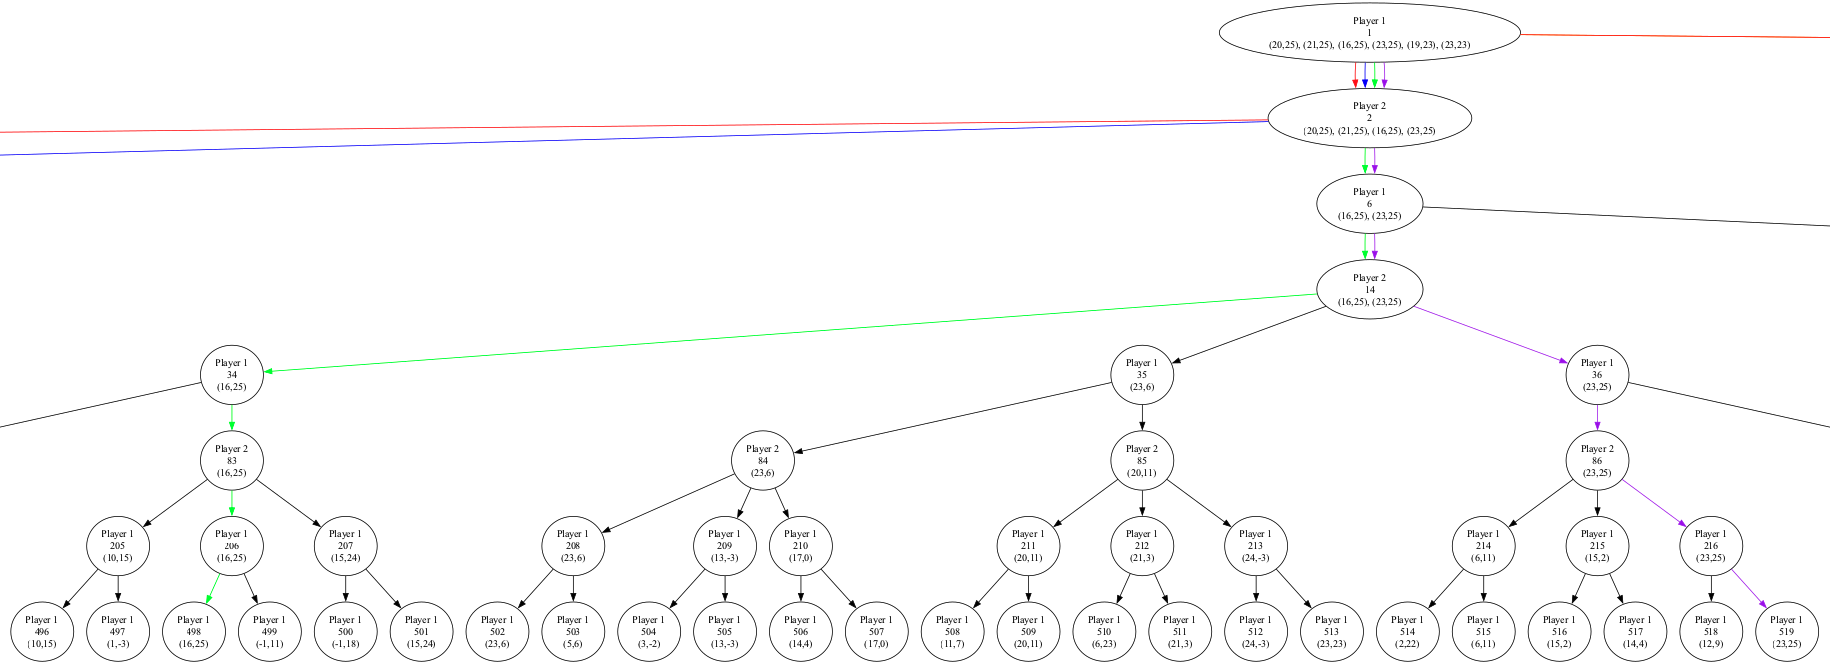
\includegraphics[scale=0.3]{../../artifacts/lw4/3.png}
  \caption{Итоговая оптимальная стратегия}
  \label{fig:fig03}
\end{figure}

На рисунке~\ref{fig:fig03} показаны, как игроки делают выбор на основе уже агрегированных
выигрышей, полученных из нижележащих уровней. Таким образом в 14 узле выбираются все
кортежи из 34 и 36 узлов, потому что при ходе второго игрока в узлах одинаковые элементы
-- 25.

\begin{figure}
  \centering
  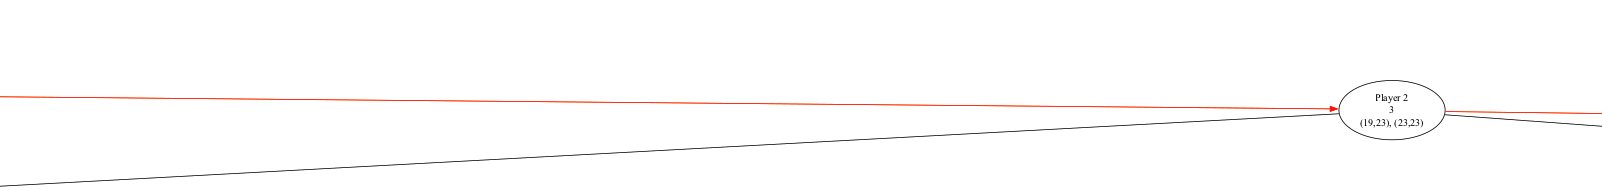
\includegraphics[scale=0.3]{../../artifacts/lw4/4.png}
  \caption{Второй дочерний узел корня}
  \label{fig:fig04}
\end{figure}

Итоговая оптимальная стратегия состоит из всех стратегий узла 2 (см.
рисунок~\ref{fig:fig03}) и узла 3, который показан на рисунке~\ref{fig:fig04} за счет
того, что при ходе первого игрока максимальный элемент 23 находится как во 2, так и в 3
узлах.

Итого, все пути, разукрашенные в цвета, отличные от черного и дошедшие до корня,
являются решениями игры. Выигрышими являются кортежи (20, 25), (21, 25), (16, 25),
(23, 25), (19, 23), (23, 23).
